%                        "      m           ""#                  mmm
%  mmm    mmm   mmmm   mmm    mm#mm  m   m    #     mmm            #
% #"  "  "   #  #" "#    #      #    #   #    #    #" "#           #
% #      m"""#  #   #    #      #    #   #    #    #   #           #
% "#mm"  "mm"#  ##m#"  mm#mm    "mm  "mm"#    "mm  "#m#"         mm#mm
%               #
%               "
\chapter{Introdução}

% Objetivo - Construir um sistema computacional completo (hardware, software
%            básico, aplicação) para máquinas de instrução única (OISC)

% Inserir alguma citação de artigo ou livro falando sobre a evolução
% dos computadores.
Com o aumento na capacidade de processamento dos computadores modernos,
aumenta-se a complexidade de seus componentes internos. As arquiteturas de
computadores modernos possuem mais instruções que as de computadores antigos,
devido à refinação do \textit{hardware}.

Em contrapartida, existem computadores com conjunto reduzido de instruções
(\textit{RISC}) e até máquinas com apenas uma única instrução
(\textit{OISC}). Esse trabalho se concentra no segundo, mais especificamente na
máquina de instrução única \textit{SUBLEQ}.

Esse trabalho visa desenvolver um sistema computacional completo
(\textit{hardware}, \textit{software} básico e \textit{software} de aplicação)
baseado na arquitetura de instrução única \textit{SUBLEQ}. Dentre as aplicações
possíveis, esperamos que o gasto de energia no processador seja constante, em
função do tempo.

% Colocar alguma coisa sobre criptografia?

Vamos explorar os conceitos básicos que levem ao objetivo final.

\section{Conceitos Básicos}

% Começando do básico do básico do básico

Computadores são sistemas incrivelmente complexos. Inúmeros componentes com
papeis específicos necessitam se intercomunicar para executar a mais simples das
tarefas. Dessa forma, para compreender seu funcionamento, se faz o uso de
camadas de abstrações.

% Camadas de abstrações
Essas camadas exercem funções diferentes e são visíveis de acordo com seu uso
--- um usuário final não precisa saber programar para usar um processador de
texto; da mesma forma, um programador não necessita saber da estrutura dos
circuitos internos. Cada camada possui seu domínio, sendo as mais próximas do
usuário final denominadas de ``alto-nível'' e as mais próximas dos transistores
e fios, ``baixo-nível''. Observe a figura \ref{camadas}, especificada de acordo
com Murdocca \cite{principles}.

% As várias camadas bonitinhas
\begin{figure}[ptb]
  \begin{center}
    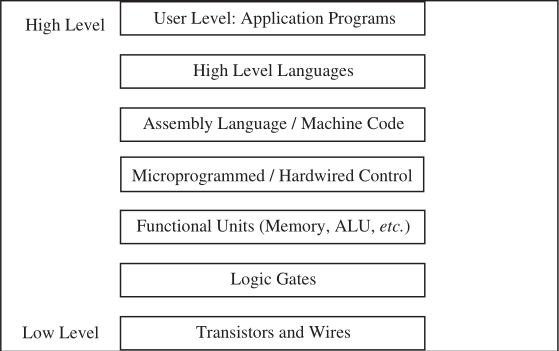
\includegraphics[scale=.6]{imagens/1_camadas}
  \end{center}
  \caption{Camadas de abstração de um computador.}
  \label{camadas}
\end{figure}

% Arquitetura do Computador -> ISA

Uma definição muito importante para o programador de sistema é a Arquitetura do
Conjunto de Instruções (\textit{Instruction Set Arquitecture}) --- de agora em
diante referida apenas como arquitetura, ou \textit{ISA}. Hennessy a define como
``o limite entre \textit{software} e \textit{hardware}'' \cite{hennessy}.

% Componentes da ISA
% (devo definir o que é "programa de sistema"?)
A \textit{ISA} descreve vários componentes essenciais para a criação de
programas de sistema. Seu \textit{design} define a memória interna do
processador, o endereçamento de memória interna e externa, quais
instruções/operações são suportadas, tipos e tamanhos de operandos, dentre
muitos outros  \cite{patterson}.

Existem tipos diferentes de \textit{ISA}, sendo comuns as arquiteturas
\textit{RISC} e \textit{CISC}.

% ISA -> RISC e CISC
Arquiteturas \textit{RISC} (\textit{Reduced Instruction Set Computer}) possuem
uma quantidade reduzida de instruções. Em geral são instruções simples e rápidas
que têm de ser combinadas para ações mais complexas. Já arquiteturas
\textit{CISC} (\textit{Complex Instruction Set Computer}) provêem uma quantidade
maior de instruções, que nativamente executam ações mais complicadas e
abrangentes.

% Vantagens da RISC
Instruções da arquitetura \textit{RISC} são mais simples; elas partem da
filosofia de otimizar os casos frequentes, visando tornar o comportamento geral
mais rápido. Murdocca argumenta que um conjunto de instruções mais simples
resulta numa central de processamento simples e menor, liberando espaço no
processador para outros componentes, como registradores \cite{principles}.

% Desvantagens da RISC
Porém Mostafa argumenta que isso traz a desvantagem de que uma grande quantidade
de instruções são necessárias para executar uma função simples \cite{mostafa},
possivelmente reduzindo o desempenho geral. Por fim, isso tambem causa um
problema cognitivo, já que programas \textit{RISC} tendem a ser mais verbosos e
depositarem a complexidade do programa nos ombros do programador.

% OISC
Além de ambas as \textit{ISA}s citadas acima, existe a arquitetura \textit{OISC}
(\textit{One Instruction Set Computer}). Ela define computadores com apenas uma
única instrução. De acordo com Gilreath, \textit{OISC} é como um \textit{CISC}
em um nível mais alto de abstração, já que precisa-se combinar essa única
instrução de diversas formas para sintetizar o que seriam as instruções mais
complexas \cite{minimalist}.

% Será que eu devo falar sobre coisas Turing-completas?
% Como OISC são equivalentes às RISC/CISC nesse sentido?

% Mesmas desvantagens de RISC
Pela própria definição, arquiteturas \textit{OISC} possuem as desvantagens de
\textit{RISC} em escala muito maior. Qualquer função simples necessitará de
várias combinações da única instrução, dificultando tanto a velocidade quanto
compreensão do programa final.

Entretanto, existem vantagens na previsibilidade de máquinas \textit{OISC}.

% Dar introdução à criptografia?

% CISC/RISC, gasto de energia diferente
Em máquinas não-\textit{OISC}, existe um conjunto bem-definido de instruções que
podem ser executadas. Cada uma exige demandas específicas do processador,
resultando em gastos de energia possivelmente diferentes.

% Olhando o gasto de energia, deduzir instruções.
% (CITAÇÃO AQUI?)
Dessa forma, ao se monitorar o gasto de energia por um período suficiente de
tempo, pode-se observar os padrões de gasto de energia do processador. Então, um
observador externo poderá deduzir quais instruções foram executadas na máquina
sem necessariamente ter acesso à mesma.

Considerando que arquiteturas \textit{OISC} possuem apenas uma instrução, cuja
demanda ao processador é única, assume-se que o gasto de energia será
constante. Logo, não seria possível determinar quais ações essa máquina executou
independentemente da quantidade de tempo de monitoramento.

% Gasto de energia deve ser constante
O ponto abordado nesse trabalho é exatamente esse --- determinar se o gasto de
energia em função do tempo é constante numa máquina \textit{OISC}. Se for o
caso, pode-se determinar aplicações interessantes para esse tipo de computador
na área de segurança de informação e criptografia.

Primeiramente, devemos determinar que instrução será usada na nossa máquina
\textit{OISC}.

\section{Linguagem de Montagem Subleq}
\label{sec:subleq}

Existem várias máquinas de arquitetura \textit{OISC}. Uma delas é a máquina que
possui apenas a instrução \textit{SUBLEQ} (\textit{Subtract and Branch on Less
  or Equal} \cite{subleq}.

% Pontos positivos
% * Previsibilidade
% Pontos negativos
% * Impacto na velocidade de execução

